% Generated by Sphinx.
\documentclass[letterpaper,10pt,english]{manual}
\usepackage[utf8]{inputenc}
\usepackage[T1]{fontenc}
\usepackage{babel}
\usepackage{times}
\usepackage[Bjarne]{fncychap}
\usepackage{longtable}
\usepackage{sphinx}


\title{Online Management GUI Documentation}
\date{October 26, 2009}
\release{0.1}
\author{Corey Oordt}
\newcommand{\sphinxlogo}{}
\renewcommand{\releasename}{Release}
\makeindex
\makemodindex

\makeatletter
\def\PYG@reset{\let\PYG@it=\relax \let\PYG@bf=\relax%
    \let\PYG@ul=\relax \let\PYG@tc=\relax%
    \let\PYG@bc=\relax \let\PYG@ff=\relax}
\def\PYG@tok#1{\csname PYG@tok@#1\endcsname}
\def\PYG@toks#1+{\ifx\relax#1\empty\else%
    \PYG@tok{#1}\expandafter\PYG@toks\fi}
\def\PYG@do#1{\PYG@bc{\PYG@tc{\PYG@ul{%
    \PYG@it{\PYG@bf{\PYG@ff{#1}}}}}}}
\def\PYG#1#2{\PYG@reset\PYG@toks#1+\relax+\PYG@do{#2}}

\def\PYG@tok@gd{\def\PYG@tc##1{\textcolor[rgb]{0.63,0.00,0.00}{##1}}}
\def\PYG@tok@gu{\let\PYG@bf=\textbf\def\PYG@tc##1{\textcolor[rgb]{0.50,0.00,0.50}{##1}}}
\def\PYG@tok@gt{\def\PYG@tc##1{\textcolor[rgb]{0.00,0.25,0.82}{##1}}}
\def\PYG@tok@gs{\let\PYG@bf=\textbf}
\def\PYG@tok@gr{\def\PYG@tc##1{\textcolor[rgb]{1.00,0.00,0.00}{##1}}}
\def\PYG@tok@cm{\let\PYG@it=\textit\def\PYG@tc##1{\textcolor[rgb]{0.25,0.50,0.56}{##1}}}
\def\PYG@tok@vg{\def\PYG@tc##1{\textcolor[rgb]{0.73,0.38,0.84}{##1}}}
\def\PYG@tok@m{\def\PYG@tc##1{\textcolor[rgb]{0.13,0.50,0.31}{##1}}}
\def\PYG@tok@mh{\def\PYG@tc##1{\textcolor[rgb]{0.13,0.50,0.31}{##1}}}
\def\PYG@tok@cs{\def\PYG@tc##1{\textcolor[rgb]{0.25,0.50,0.56}{##1}}\def\PYG@bc##1{\colorbox[rgb]{1.00,0.94,0.94}{##1}}}
\def\PYG@tok@ge{\let\PYG@it=\textit}
\def\PYG@tok@vc{\def\PYG@tc##1{\textcolor[rgb]{0.73,0.38,0.84}{##1}}}
\def\PYG@tok@il{\def\PYG@tc##1{\textcolor[rgb]{0.13,0.50,0.31}{##1}}}
\def\PYG@tok@go{\def\PYG@tc##1{\textcolor[rgb]{0.19,0.19,0.19}{##1}}}
\def\PYG@tok@cp{\def\PYG@tc##1{\textcolor[rgb]{0.00,0.44,0.13}{##1}}}
\def\PYG@tok@gi{\def\PYG@tc##1{\textcolor[rgb]{0.00,0.63,0.00}{##1}}}
\def\PYG@tok@gh{\let\PYG@bf=\textbf\def\PYG@tc##1{\textcolor[rgb]{0.00,0.00,0.50}{##1}}}
\def\PYG@tok@ni{\let\PYG@bf=\textbf\def\PYG@tc##1{\textcolor[rgb]{0.84,0.33,0.22}{##1}}}
\def\PYG@tok@nl{\let\PYG@bf=\textbf\def\PYG@tc##1{\textcolor[rgb]{0.00,0.13,0.44}{##1}}}
\def\PYG@tok@nn{\let\PYG@bf=\textbf\def\PYG@tc##1{\textcolor[rgb]{0.05,0.52,0.71}{##1}}}
\def\PYG@tok@no{\def\PYG@tc##1{\textcolor[rgb]{0.38,0.68,0.84}{##1}}}
\def\PYG@tok@na{\def\PYG@tc##1{\textcolor[rgb]{0.25,0.44,0.63}{##1}}}
\def\PYG@tok@nb{\def\PYG@tc##1{\textcolor[rgb]{0.00,0.44,0.13}{##1}}}
\def\PYG@tok@nc{\let\PYG@bf=\textbf\def\PYG@tc##1{\textcolor[rgb]{0.05,0.52,0.71}{##1}}}
\def\PYG@tok@nd{\let\PYG@bf=\textbf\def\PYG@tc##1{\textcolor[rgb]{0.33,0.33,0.33}{##1}}}
\def\PYG@tok@ne{\def\PYG@tc##1{\textcolor[rgb]{0.00,0.44,0.13}{##1}}}
\def\PYG@tok@nf{\def\PYG@tc##1{\textcolor[rgb]{0.02,0.16,0.49}{##1}}}
\def\PYG@tok@si{\let\PYG@it=\textit\def\PYG@tc##1{\textcolor[rgb]{0.44,0.63,0.82}{##1}}}
\def\PYG@tok@s2{\def\PYG@tc##1{\textcolor[rgb]{0.25,0.44,0.63}{##1}}}
\def\PYG@tok@vi{\def\PYG@tc##1{\textcolor[rgb]{0.73,0.38,0.84}{##1}}}
\def\PYG@tok@nt{\let\PYG@bf=\textbf\def\PYG@tc##1{\textcolor[rgb]{0.02,0.16,0.45}{##1}}}
\def\PYG@tok@nv{\def\PYG@tc##1{\textcolor[rgb]{0.73,0.38,0.84}{##1}}}
\def\PYG@tok@s1{\def\PYG@tc##1{\textcolor[rgb]{0.25,0.44,0.63}{##1}}}
\def\PYG@tok@gp{\let\PYG@bf=\textbf\def\PYG@tc##1{\textcolor[rgb]{0.78,0.36,0.04}{##1}}}
\def\PYG@tok@sh{\def\PYG@tc##1{\textcolor[rgb]{0.25,0.44,0.63}{##1}}}
\def\PYG@tok@ow{\let\PYG@bf=\textbf\def\PYG@tc##1{\textcolor[rgb]{0.00,0.44,0.13}{##1}}}
\def\PYG@tok@sx{\def\PYG@tc##1{\textcolor[rgb]{0.78,0.36,0.04}{##1}}}
\def\PYG@tok@bp{\def\PYG@tc##1{\textcolor[rgb]{0.00,0.44,0.13}{##1}}}
\def\PYG@tok@c1{\let\PYG@it=\textit\def\PYG@tc##1{\textcolor[rgb]{0.25,0.50,0.56}{##1}}}
\def\PYG@tok@kc{\let\PYG@bf=\textbf\def\PYG@tc##1{\textcolor[rgb]{0.00,0.44,0.13}{##1}}}
\def\PYG@tok@c{\let\PYG@it=\textit\def\PYG@tc##1{\textcolor[rgb]{0.25,0.50,0.56}{##1}}}
\def\PYG@tok@mf{\def\PYG@tc##1{\textcolor[rgb]{0.13,0.50,0.31}{##1}}}
\def\PYG@tok@err{\def\PYG@bc##1{\fcolorbox[rgb]{1.00,0.00,0.00}{1,1,1}{##1}}}
\def\PYG@tok@kd{\let\PYG@bf=\textbf\def\PYG@tc##1{\textcolor[rgb]{0.00,0.44,0.13}{##1}}}
\def\PYG@tok@ss{\def\PYG@tc##1{\textcolor[rgb]{0.32,0.47,0.09}{##1}}}
\def\PYG@tok@sr{\def\PYG@tc##1{\textcolor[rgb]{0.14,0.33,0.53}{##1}}}
\def\PYG@tok@mo{\def\PYG@tc##1{\textcolor[rgb]{0.13,0.50,0.31}{##1}}}
\def\PYG@tok@mi{\def\PYG@tc##1{\textcolor[rgb]{0.13,0.50,0.31}{##1}}}
\def\PYG@tok@kn{\let\PYG@bf=\textbf\def\PYG@tc##1{\textcolor[rgb]{0.00,0.44,0.13}{##1}}}
\def\PYG@tok@o{\def\PYG@tc##1{\textcolor[rgb]{0.40,0.40,0.40}{##1}}}
\def\PYG@tok@kr{\let\PYG@bf=\textbf\def\PYG@tc##1{\textcolor[rgb]{0.00,0.44,0.13}{##1}}}
\def\PYG@tok@s{\def\PYG@tc##1{\textcolor[rgb]{0.25,0.44,0.63}{##1}}}
\def\PYG@tok@kp{\def\PYG@tc##1{\textcolor[rgb]{0.00,0.44,0.13}{##1}}}
\def\PYG@tok@w{\def\PYG@tc##1{\textcolor[rgb]{0.73,0.73,0.73}{##1}}}
\def\PYG@tok@kt{\def\PYG@tc##1{\textcolor[rgb]{0.56,0.13,0.00}{##1}}}
\def\PYG@tok@sc{\def\PYG@tc##1{\textcolor[rgb]{0.25,0.44,0.63}{##1}}}
\def\PYG@tok@sb{\def\PYG@tc##1{\textcolor[rgb]{0.25,0.44,0.63}{##1}}}
\def\PYG@tok@k{\let\PYG@bf=\textbf\def\PYG@tc##1{\textcolor[rgb]{0.00,0.44,0.13}{##1}}}
\def\PYG@tok@se{\let\PYG@bf=\textbf\def\PYG@tc##1{\textcolor[rgb]{0.25,0.44,0.63}{##1}}}
\def\PYG@tok@sd{\let\PYG@it=\textit\def\PYG@tc##1{\textcolor[rgb]{0.25,0.44,0.63}{##1}}}

\def\PYGZat{@}
\def\PYGZlb{[}
\def\PYGZrb{]}
\makeatother

\begin{document}

\maketitle
\tableofcontents
\hypertarget{--doc-index}{}


Contents:

\resetcurrentobjects
\hypertarget{--doc-goals}{}

\chapter{Goals}
\begin{enumerate}
\item {} 
Specify website requirements by:
\begin{itemize}
\item {} 
Package requirements on the server

\item {} 
Language-specific library requirements

\end{itemize}

\item {} 
Configure a server by specifying base requirements

\item {} 
Deploy a web site to a server:
\begin{itemize}
\item {} 
Install all server and language dependencies on the server

\item {} 
Copy site to server in one of several methods:
\begin{itemize}
\item {} 
VCS checkout

\item {} 
tar.gzip

\item {} 
rsync

\end{itemize}

\end{itemize}

\item {} 
Update one or more files on a web site via same methods as deployment

\item {} 
Allow for multiple types of server operating systems, as long as they have a package manager to install packages

\end{enumerate}

\resetcurrentobjects
\hypertarget{--doc-gettingstarted/creating_serveros}{}

\hypertarget{gettingstarted-creating-serveros}{}\chapter{Creating a Server OS}

The server operating system is where the implementation of services is described. It also describes how services are installed and how you can tell if a service is in fact installed.

There are three parts to defining a Server OS: \hyperlink{howthingsaredone}{\emph{Defining ``How Things are Done''}}, \hyperlink{howservicesareinstalled}{\emph{Defining ``How Services are Installed''}}, and \hyperlink{howaservicecommandsareexecuted}{\emph{Defining ``How a Service Commands are Executed''}}.


\hypertarget{howthingsaredone}{}\section{Defining ``How Things are Done''}
\begin{enumerate}
\item {} 
In the admin, click the \textbf{Add} button on the \textbf{ServerOSes} line.

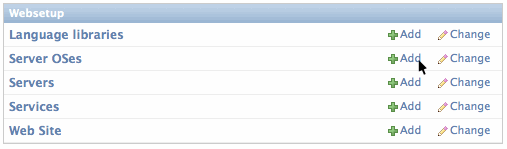
\includegraphics[width=507pt,height=149pt]{add_serveros.png}

\item {} 
In the top part of the form, enter the name of the operating system, the command to install a package and the command to find if a package is installed. The commands can use the placeholder \code{\%(package)s} for the package name; multiple times if necessary.

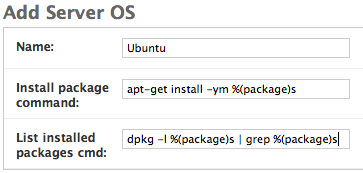
\includegraphics[width=363pt,height=173pt]{add_serveros_form.png}

In this case, \code{Ubunutu}, the command to install a package is \code{apt-get install -ym \%(package)s}. The command to find whether or not a package is installed is more complex. The command to list all installed packages \code{dpkg -l \%(package)s} is piped (\code{\textbar{}}) through \code{grep \%(package)s} to find the package name in the list.

\end{enumerate}
\hypertarget{howservicesareinstalled}{}

\section{Defining ``How Services are Installed''}
\begin{enumerate}
\item {} 
Select the service from the popup menu in the \textbf{Service} column.

\item {} 
Type in the name of the package or packages that are required to implement this service on this ServerOS in the \textbf{Package} column. Separate packages by spaces.

For example, to implement \code{Apache 2.2} on \code{Ubuntu}, the packages required are: \code{apache2.2-common apache2-mpm-worker apache2-utils apache2 libapache2-mod-wsgi}.

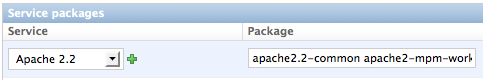
\includegraphics[width=483pt,height=80pt]{add_service_package.png}

\end{enumerate}
\hypertarget{howaservicecommandsareexecuted}{}

\section{Defining ``How a Service Commands are Executed''}
\begin{enumerate}
\item {} 
Select the service's command from the popup menu in the \textbf{Command} column.

\item {} 
Type in the command to execute it on this Server OS in the \textbf{Command string} column.

\item {} 
Make sure the checkbox in the \textbf{Must sudo} column is checked (the default) if this command must be executed with superuser privileges, or unchecked if it does not.

For example to implement the \code{Apache 2.2 start} command on \code{Ubuntu}, the string \code{/etc/init.d/apache2 start} must be executed with superuser privileges.

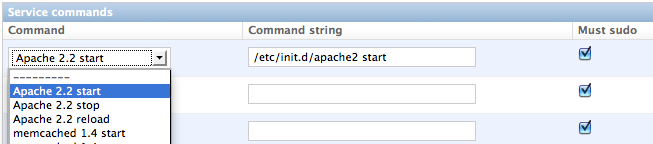
\includegraphics[width=653pt,height=144pt]{add_service_command.png}

\end{enumerate}

\resetcurrentobjects
\hypertarget{--doc-gettingstarted/creating_services}{}

\hypertarget{gettingstarted-creating-services}{}\chapter{Creating Services}

Services are very simple to create. When you define a service, you will also define the commands that apply to the service, such as start, stop, and reload.

You are not going to enter any installation or execution information here. That information is entered in each \hyperlink{models-serveros}{\emph{Server OS}}.
\begin{enumerate}
\item {} 
In the admin, click the \textbf{Add} button on the \textbf{Service} line.

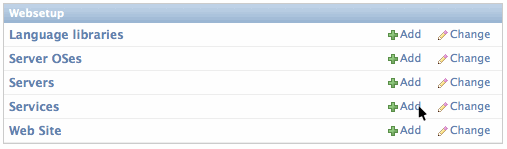
\includegraphics{add_service1.png}

\item {} 
Fill out the the \textbf{Name} field and optionally enter a description in the \textbf{Description} field.

\item {} 
Enter up to three commands for the service and optionally a description of what the command does.

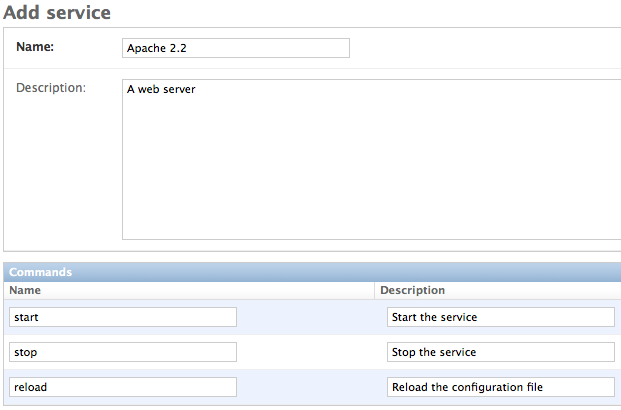
\includegraphics{add_service_form.png}

\begin{notice}{note}{Note:}
If you want to add more commands, click on the \textbf{Save and Continue Editing} button instead of \textbf{Save}. When you are done entering commands, click the \textbf{Save} button.
\end{notice}

\item {} 
Click on the \textbf{Save} button.

\end{enumerate}

\resetcurrentobjects
\hypertarget{--doc-models}{}

\hypertarget{models}{}\chapter{Models}
\begin{figure}[htbp]
\centering

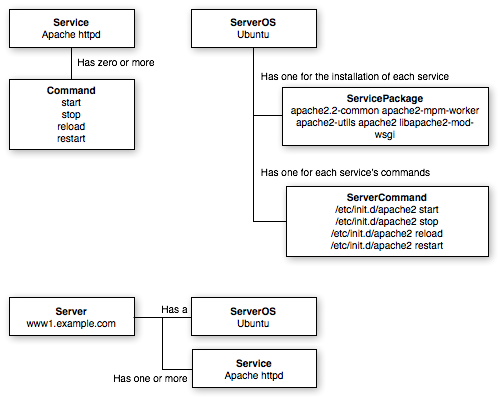
\includegraphics{OMG_schema_example1.png}
\caption{Here is a simple diagram of the how the classes connect, using example data
to help illustrate the connections}\end{figure}


\hypertarget{models-service}{}\section{Services and Commands}

\emph{Services} are processes like Apache httpd, memcached and the like. A service may have \emph{Commands} to do things like start it, stop it, and reload its configuration.

For example \textbf{Service} Apache httpd has \textbf{Command}s start, stop, reload, status, and config\_test.

Services and commands do not include any implementation information. All implementation is done in the \hyperlink{models-serveros}{\emph{ServerOS}}.
\hypertarget{models-serveros}{}

\section{ServerOS, ServicePackage and ServiceCommand}

An operating system for a server. The ServerOS describes how to install system packages (using apt or yum for example), which packages are required
\hypertarget{models-servicepackage}{}

\section{ServicePackage}

The package or packages required to install the \hyperlink{models-service}{\emph{Service}} on to the \hyperlink{models-serveros}{\emph{Server Operating System}}. Installation of the Service will use the package manager commands indicated in the Server Operating System.
\hypertarget{models-servicecommand}{}

\section{ServiceCommand}

Commands for services based on the operating system.
\hypertarget{models-languagelibrary}{}

\section{LanguageLibrary}

A library for a language, typically installed with a language-specific tool
\hypertarget{models-server}{}

\section{Server}

A machine with services and web sites.
\hypertarget{models-website}{}

\section{WebSite}

A web site that is on one or more servers

\resetcurrentobjects
\hypertarget{--doc-reference/models}{}

\chapter{Model Reference}


\chapter{Indices and tables}
\begin{itemize}
\item {} 
\emph{Index}

\item {} 
\emph{Module Index}

\item {} 
\emph{Search Page}

\end{itemize}


\renewcommand{\indexname}{Module Index}
\printmodindex
\renewcommand{\indexname}{Index}
\printindex
\end{document}
